\documentclass[dvipdfmx,fleqn]{beamer}
%\documentclass[dvipdfmx,fleqn,handout]{beamer}
\usepackage{amsmath,amssymb,amsthm}

\mode<presentation>
{
  \usetheme{default}
}

\title{\Large タイトル}
\author{\large 名前}
\date{\small 日付}

\usefonttheme{professionalfonts}

\setbeamercovered{transparent=20}

\setbeamertemplate{navigation symbols}{} 
\setbeamertemplate{footline}[frame number] 



\begin{document}

\sffamily
\gtfamily


\begin{frame}
  \titlepage
  \thispagestyle{empty}
\end{frame}

\setcounter{framenumber}{0}




\begin{frame}
\frametitle{はじめに}
\begin{itemize}\setlength{\parskip}{0.5em}
\item
項目1

\item
項目2
 \begin{itemize}\setlength{\parskip}{0.5em}
 \item
 1階層下の項目1
 \item
 1階層下の項目2
 \end{itemize}

\item
このページの最後の項目
\end{itemize}
\end{frame}



\begin{frame}
\frametitle{次のスライド}
\begin{itemize}\setlength{\parskip}{0.5em}
\item
Ficititious playの説明1

\item
Ficititious playの説明2 \pause

$x_0(t)$ は
\[
x_0(t+1)
= x_0(t) + \frac{1}{t+2} (a_1(t) - x_0(t))
\]
と再帰的に書くことができる. \pause

\item
Ficititious playの説明3 \pause

\item
``\texttt{pause}''をつけるとoverlayができる.

\item
ファイルの冒頭の\texttt{documentclass}のオプションで\texttt{handout}を指定すると,
overlayにならずいっぺんに表示される.

Webにのせるときや,印刷して配るときなどは\texttt{handout}を指定しておく.

\end{itemize}
\end{frame}



\begin{frame}[containsverbatim]% verbatim 環境を使えるように
\frametitle{コードの説明とか}
\begin{itemize}\setlength{\parskip}{0.5em}
\item
コードの表示の例
\begin{verbatim}
 1: import matplotlib.pyplot as plt
 2: import random
 3: import numpy as np
 4: 
 5: 
 6: class FP:
 7: 
 8:     def __init__(self, profits):
 9:         self.pro = profits
10:         self.cu_xs = [0, 0]
11:         self.x0s = []
12:         self.x1s = []
13:         pro_cal = (np.transpose(self.pro)[0],
14:                    np.transpose(np.transpose(self.pro)[1]))
15:         self.x0s = []
16:         self.x1s = []
17:         self.cu_xs = [random.uniform(0, 1), random.uniform(0, 1)]
18:         cu_es = [[0, 0], [0, 0]]
19:         for i in range(ts_length):
20:             self.x0s.append(self.cu_xs[0])
21:             self.x1s.append(self.cu_xs[1])
22:             exp = ((1-self.cu_xs[0], self.cu_xs[0]),
23:                    (1-self.cu_xs[1], self.cu_xs[1]))
24:             cu_es[0] = np.dot(pro_cal[0], exp[0])
25:             cu_es[1] = np.dot(pro_cal[1], exp[1])
26:             cu_as = [0, 0]  # the act of players
27:             for j in range(2):
28:                 if cu_es[j][0] == cu_es[j][1]:
29:                     cu_as[j] = random.randint(0, 1)
30:                 else:
31:                     cu_as[j] = cu_es[j].argmax()
32:             for k in range(2):
33:                 self.cu_xs[k] = (self.cu_xs[k]*(i+1)+cu_as[1-k])/(i+2)
34: 
35:     def playplot(self, ts_length):
36:         self.oneplay(ts_length)
37:         plt.plot(self.x0s, 'b-', label='x_0(t)')  # blue line means x_0(t)
38:         plt.plot(self.x1s, 'r-', label='x_1(t)')  # red line means x_1(t)
39:         plt.legend()
40         plt.show()
41: 
42:     def playsave(self, ts_length, name):  # name is str
43:         self.oneplay(ts_length)
44:         plt.plot(self.x0s, 'b-', label='x_0(t)')  # blue line means x_0(t)
45:         plt.plot(self.x1s, 'r-', label='x_1(t)')  # red line means x_1(t)
46:         plt.legend()
47:         plt.savefig(str(name)+'.png', bbox_inches='tight', pad_inches=0)
48:         plt.savefig(str(name)+'.pdf', bbox_inches='tight', pad_inches=0)
49:         plt.close()
50: 
51:     def histogram(self, n, ts_length):
52:         last_x0s = []
53:         for j in range(n):
54:             self.oneplay(ts_length)
55:             last_x0s.append(self.cu_xs[0])
56:         ax = plt.subplot(111)
57:         ax.hist(last_x0s, alpha=0.6, bins=5)
58:         ax.set_xlim(xmin=0, xmax=1)
59:         t = 'ts = '+str(ts_length)+', times = '+str(n)
60:         ax.set_title(t)
61: 
62:     def histplot(self, n, ts_length):
63:         self.histogram(n, ts_length)
64:         plt.show()
65: 
66:     def histsave(self, n, ts_length, name):
67:         self.histogram(n, ts_length)
68:         plt.savefig(str(name)+'.png', bbox_inches='tight', pad_inches=0)
69:         plt.savefig(str(name)+'.pdf', bbox_inches='tight', pad_inches=0)
70:         plt.close()
\end{verbatim}

\item
\verb|\begin{frame}| から \verb|\end{frame}| までを
コピー\&ペーストしてスライドを増やしていく.
\end{itemize}
\end{frame}



\begin{frame}
\frametitle{図}
\begin{figure}
 \centering
 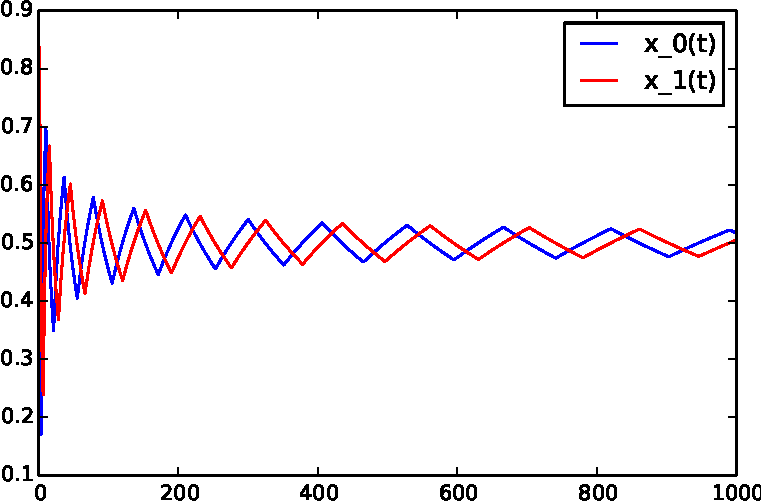
\includegraphics{oneplay2.pdf}
 \caption{図の表示}
 \label{fig:matchingpennies_plot}
\end{figure}
\end{frame}



\begin{frame}
\frametitle{まとめ}
\begin{itemize}\setlength{\parskip}{0.5em}
\item
まとめ

\item
よくわかっていない点とか

\item
今後の課題とか
\end{itemize}
\end{frame}



\end{document}